\section{Boxplots}


\begin{figure}[htbp]
	\centering
	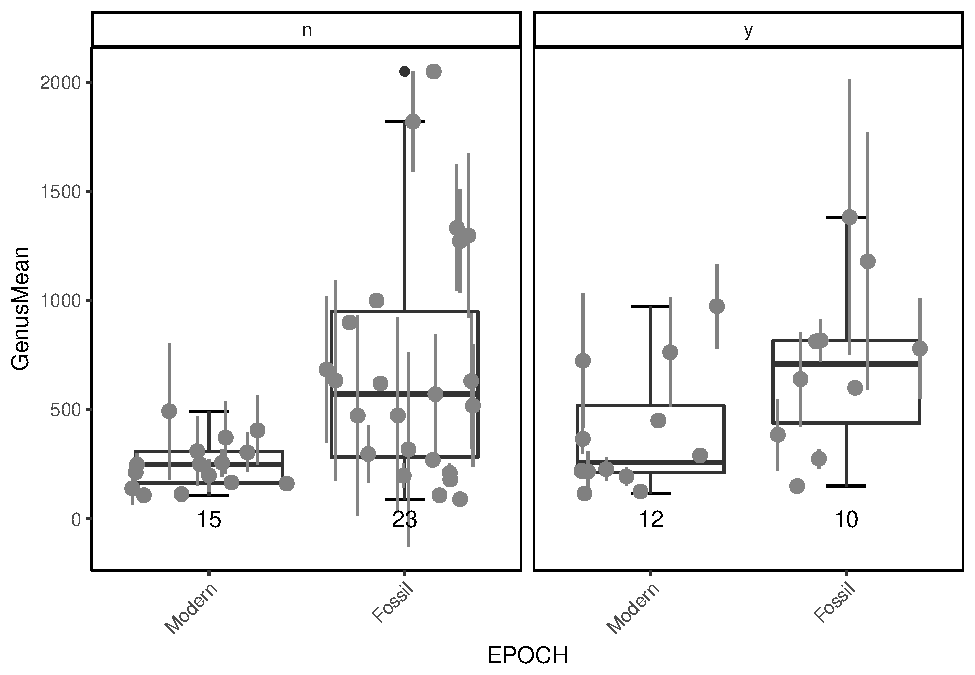
\includegraphics{MA_JJ_files/figure-latex/BPFMCI-1.pdf}
	\caption{Boxplots fossil vs.~modern, continental vs.~insular species.}
\end{figure}


Wilcoxon Rank Sum Test (unpaired data):

modern continental \textless{} fossil continental (P =
\(4.8532266\times 10^{-8}\))

modern insular \textless{} fossil insular (P = \(0.0018564\))




\begin{figure}[htbp]
	\centering
	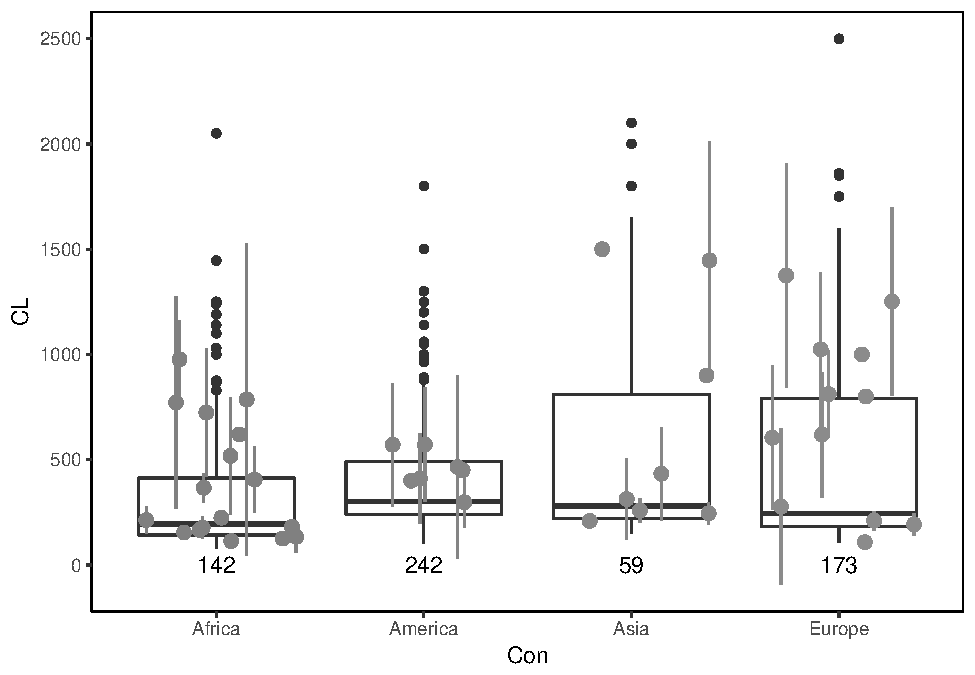
\includegraphics{MA_JJ_files/figure-latex/BPCon-1.pdf}
	\caption{Boxplot: body size on different continents, genera summarised}
\end{figure}


Kruskal-Wallis-Test:

Continent means differ (P = \(1.0833256\times 10^{-6}\)) (still have to
look into the details\ldots{})